\section{Introduction}

Applications for assembly robots have been primarily implemented in fixed and programmable automation. Fixed automation is a process using mechanized machinery to perform fixed and repetitive operations in order to produce a high volume of similar parts. Although fixed automation provides maximum efficiency at a low unit cost, drastic modifications of the machines are realized when parts need major changes or become too complicated in design. In programmable automation, products are made in batch quantities ranging from several dozen to several thousand units at a time. However, each new batch requires long set up time to accommodate the new product style. The time and therefore the cost of developing applications for fixed and programmable automation is usually quite high. The challenge of expanding industrial use of robots is through agile and flexible automation where minimized setup times can lead in to more output and generally better throughput.

The effort presented in this paper describes a methodology and tools in the area of industrial assembly of manufactured products. This effort is designed to support the IEEE Robotics and Automation Society's Ontologies for Robotics and Automation Working Group. Industrial assembly of manufactured products is often performed by first bringing parts together in a kit and then moving the kit to the assembly area where the parts are used to assemble products. Kitting is the process in which several different, but related items are placed into a container and supplied together as a single unit (kit). Kitting itself may be viewed as a specialization of the general bin-picking problem. In industrial assembly of manufactured products, kitting is often performed prior to final assembly. Agile and flexible kitting, when applied properly, has been observed to show numerous benefits for the assembly line, such as cost savings~\cite{Carlsson_2008} including saving manufacturing or assembly space~\cite{Medbo2003}, reducing assembly workers walking and searching times~\cite{Schwind1992}, and increasing line flexibility~\cite{Bozer1992} and balance~\cite{Jiao2000}.

The concept of agile manufacturing~\cite{SHERIDAN.1993,Struebing.1995,NAGEL.1991} was first introduced in 1991 at the end of a government-sponsored research effort at Lehigh University. This effort reunited a group of more than 150 industry executives to discuss the evolution of US industrial competitiveness in the next 15 years.

Many definitions of agile manufacturing have emerged during the last 30 years without being opposed or contradictory to each other~\cite{Dahmardeh.2010}. Kidd~\cite{KIDD.2000} defined agility as a way for companies to rapidly adapt to tomorrow's surprises where agile production can be considered as a structure in the company which has the ability of product developments and some business methods. For Maskell~\cite{Maskell.2001}, the three main components of agile production are customer's growth and flourish, compatibility of individuals and information, and cooperation and change ability. According to Gunasekaran~\cite{GUNASEKARAN.1999}, agile production is a new production model resulting from changes in environment which links innovations in production, information technology and communication by fundamental organizational redesigning and new marketing strategies.

Agility mainly represents the idea of ``speed and change in business environment" and consists of two main factors: 1) Responding to change in proper ways and due time and 2) Exploiting changes and taking advantage of them as opportunities~\cite{SHARIFI.1999}. Agile manufacturing demands a manufacturing system that is able to produce effectively a large variety of products and to be reconfigurable to accommodate changes in the product mix and product designs~\cite{GUNASEKARAN.1999}. Reconfigurability of manufacturing systems, product variety, velocity and flexibility in production are critical aspects to achieving and maintaining competitive advantage. The concept of agility has an impact on the design of assemblies and therefore, methodologies for the design of agile manufacturing are needed.

Some of the key words and terms linked to ``agile manufacturing" are~\cite{KIDD.2000}:
\begin{itemize}
\item Fast -- A very high speed of response to new opportunities.
\item Adaptable -- The ability to change the current approach and change direction with ease.
\item Reconfiguration -- The ability to quickly reconfigure a firm structures, facilities, organization, and technology to meet unexpected and short lived market opportunities.
\item Transformation of knowledge -- The ability to explicitly transform raw ideas into a range of competence which is then used in both products and services.
\end{itemize}

The effort described in this paper tends to move towards the ideas of a fast and adaptable system. Tasking a system sensor to retrieve information on objects of interest should be performed in a timely manner before performing any actions of the plan that require these objects of interest. Parts and components in a kitting work cell are likely susceptible to be moved during the course of time by external agents and thus, the system should be able to cope with these unexpected changes in the environment.

The organization of the remainder of this paper is as follows. Section \ref{sect:kitting} describes the simulation environment for the domain of kitting. Section \ref{sect:overview} presents an overview of the knowledge driven methodology that has been developed for this effort with a particular focus on the areas where the sensor system interacts with. Section \ref{sect:operation} details the tools and the new methodology developed to task a sensor system to retrieve information on objects of interest, and Section \ref{sect:future} presents conclusions and future work.



%A failure is any change, design, or manufacturing error that renders a component, assembly, or system incapable of performing its intended function \cite{Collins93}. In kitting, failures can occur for multiple reasons including: equipment not being set up properly, tools and/or fixtures not being properly prepared, and improper equipment maintenance. Part/component availability failures can be triggered by inaccurate information on the location of the part, part damage, incorrect part types, or part shortage due to delays in internal logistics. In order to prevent or minimize failures, a disciplined approach needs to be implemented to identify the different ways a process design can fail before impacting the productivity.
%
%Even though today's state-of-the-art industrial robots are capable of sub-millimeter accuracy \cite{RobotAccuracy}, they often lack the sensing
%necessary to detect failures and the programming required to cope with and correct the failure. This is due to the fact that they are often programmed
%by an operator using crude positional controls from a teach pendent. These teach pendent programs are highly repeatable, which provides 
%utility for large-batch, error-free operation. However, the cyclic program that repeats identical operations does not lend itself well to adaptation for 
%failure mitigation. In fact, producing a program to correct a perceived failure would require that the cell be taken off-line
%for additional human-led teach pendent programming. In addition, 
%most cells lack the ability to sense that an failure occurred and  lack programming (that would have had to be teach pendent entered) to cope
%with failure conditions, thus making it impossible for the cell to recover from failures.
%This leads to faulty products being sent down the line, and/or downtime for the cell as failures are detected and corrected.
%
%For small batch processors or other customers who must frequently change their line configuration or desire to perform complex operations
%with their robots, this frequent downtime and lack of failure correction/detection may be unacceptable. The robotic systems of tomorrow need to be capable, flexible, and agile.  
%These systems need to perform their duties at least  as well as human counterparts, be quickly re-tasked to other operations, cope with a wide 
%variety of unexpected environmental and operational changes, and be able to detect and correct errors in operation. 
%To be successful, these systems need to combine domain expertise, knowledge of their own skills and limitations, and both semantic and geometric 
%environmental information.
%
%The IEEE Robotics and Automation Society's Ontologies for Robotics and Automation Working group has taken the first steps in creating the 
%infrastructure necessary for such a system, while the Industrial Subgroup has applied this infrastructure to create a sample kit building
%system.  This work is presented in Balakirsky et al. \cite{balakirsky2013} which describes the construction of a robotic kit building
%system that is able to cope with environmental and task changes without operator intervention. This article extends that work to utilize
%the same infrastructure to allow for the detection and correction of action failures in the system.
%
%The organization of the remainder of this paper is as follows. Section \ref{sect:kitting} describes the domain of kit building. Section \ref{sect:overview} presents
%an overview of the software system architecture for the robot cell. Section \ref{sect:operation} presents results of this work, and Section \ref{sect:future} presents
%conclusions and future work.





%
%
\section{Kitting}
\label{sect:kitting}
Today's advanced manufacturing plants utilize mixed-model assembly where multiple product variants are built on the same line.  
According to Jim Tetreault, Ford’s vice president of North America Manufacturing, 
new Ford assembly facilities are able to build a full spectrum of vehicles on the same assembly line \cite{James2011}. One of the technologies that makes this possible
is the use of assembly kits.  Bozer and McGinnis \cite{Bozer1992} describe a kit as ``a specific
collection of components and/or subassemblies that together (i.e., in the same container) support one or more assembly
operations for a given product or shop order''. These  kits provide a synchronous material flow, where parts and components move to 
assembly stations in a just-in-time manner. The kits provide workers with the parts and tools that they need (which may vary from 
vehicle model to vehicle model) in the sequence that they need them. The use of kitting also allows a single delivery system to feed
multiple assembly stations thus saving manufacturing or assembly space \cite{Medbo2003} and provides an additional inspection opportunity 
that allows for the detection of part defects before they impact assembly operations. The individual operations of the station 
that builds the kits may be viewed as a specialization of the general
bin-picking problem \cite{Schyja2012} where parts are picked from one or more part bins or trays and placed into specific slots in a kit tray.

For our sample implementation, we assume that the robot cell is building one of several possible kit configurations. At execution time, the
cell has a set kit to build, but does not know the precise location of the kit tray, the part trays, or the location of individual parts in the part tray.
When a human builds a kit, they are able to inspect each part before adding it to the kit tray. This provides an additional level of quality control and
is an aspect that is desirable to have in our robotic system. During kit construction,
a robot performs a series of pick-and-place operations
in order to construct the kit. These operations include:
\begin{enumerate}
\item Pick up an empty kit and place it on the work table.
\item Pick up multiple component parts, inspect them, and place them in the kit.
\item Pick up the completed kit and place it in the full kit storage area.
\end{enumerate}
Each of these may be a compound action that includes
other actions such as end-of-arm tool changes, path planning,
and obstacle avoidance. The items that are being placed in the kit may be of varying size and shape and have various grasping and inspection
requirements.
%
\begin{figure}[htb!]
\begin{center}
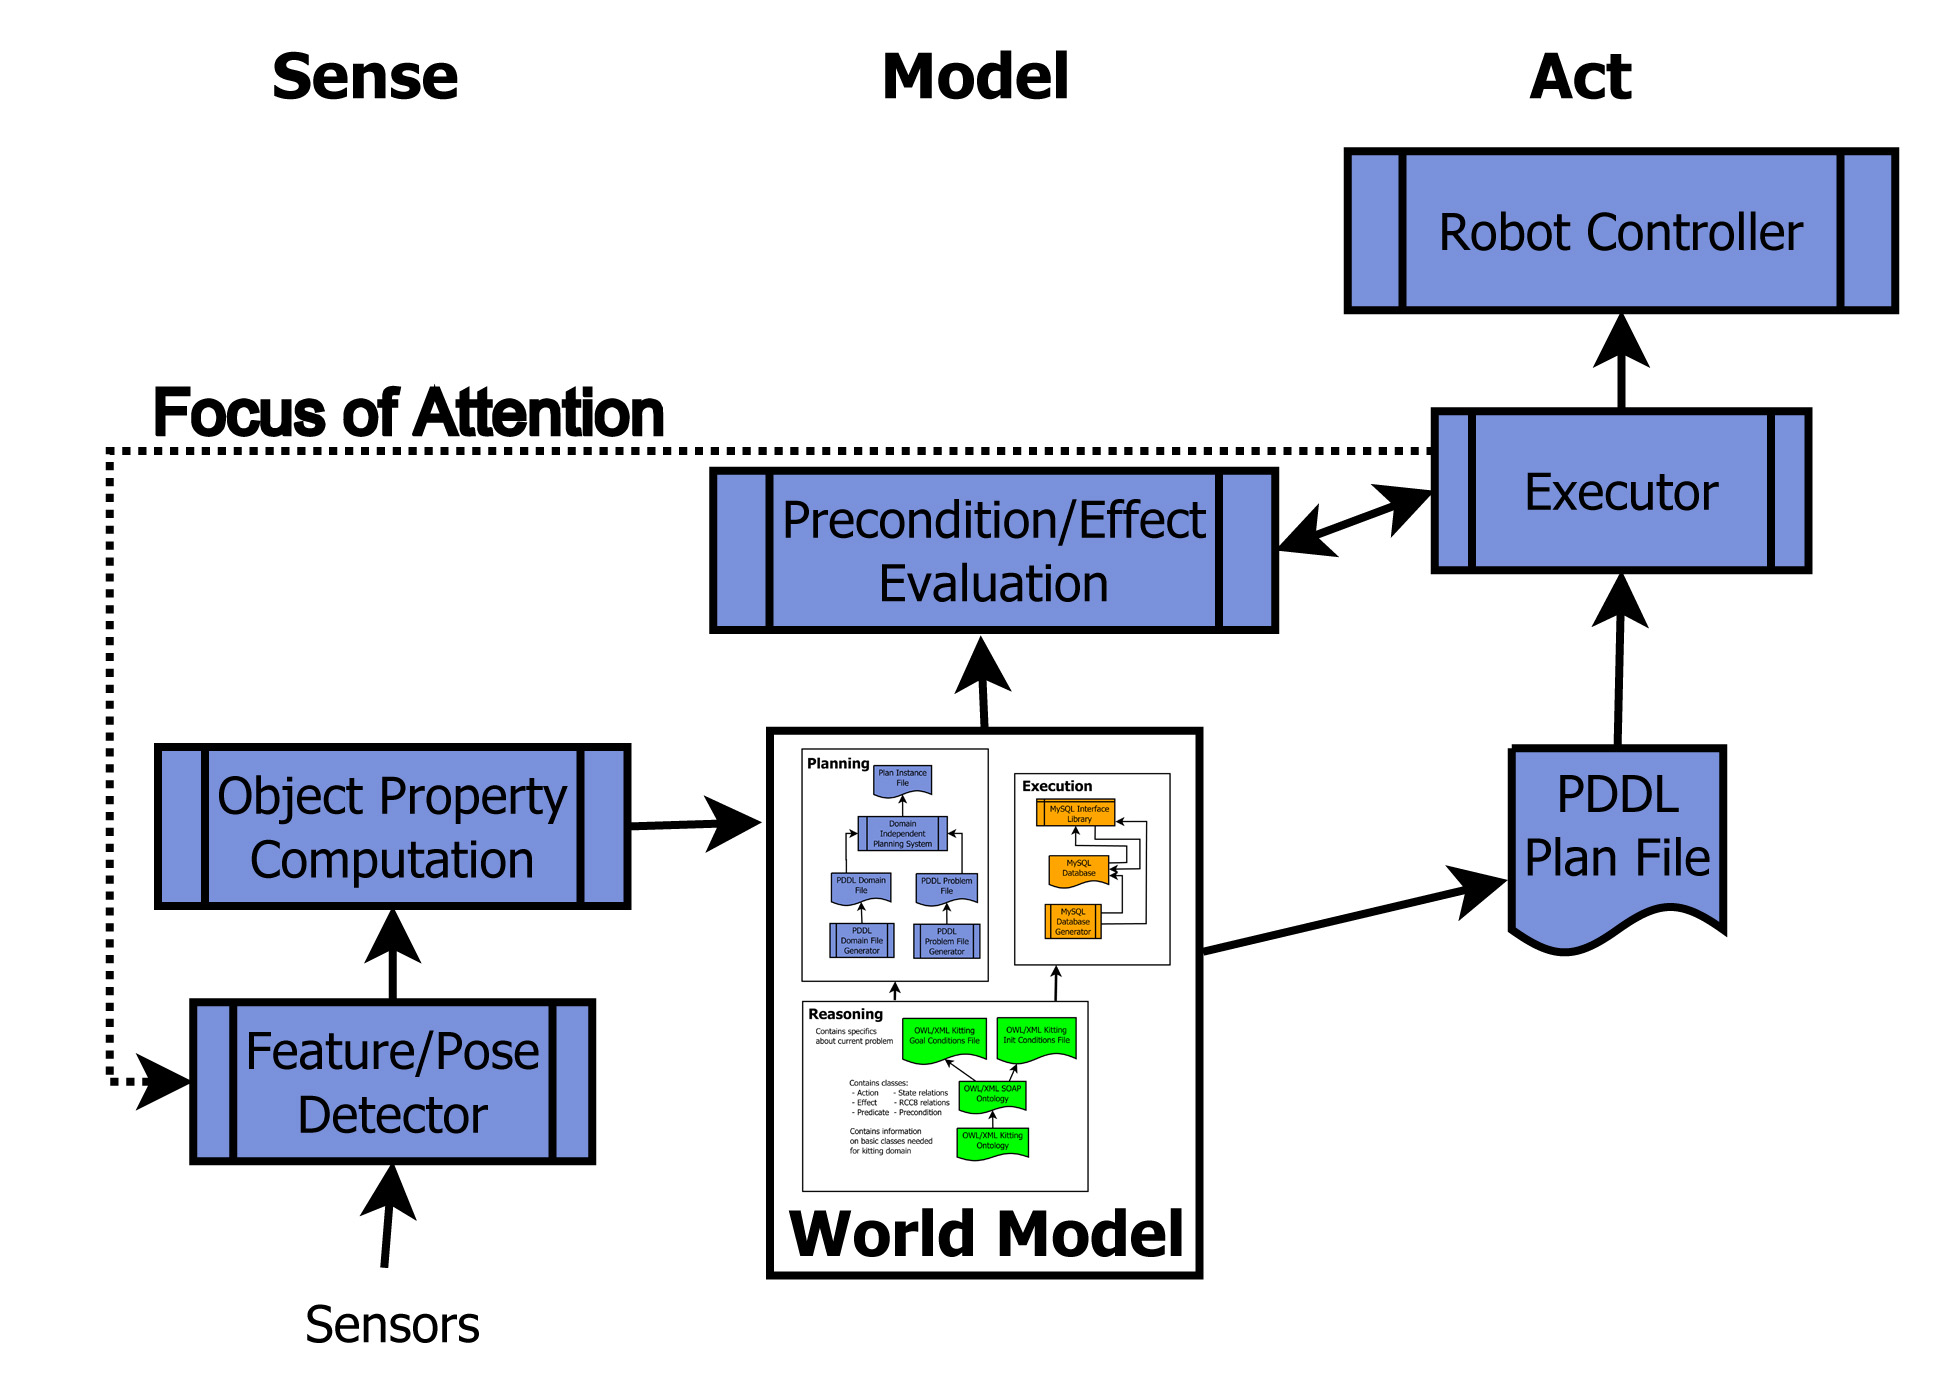
\includegraphics[width=8.5cm]{images/RITAExecution.jpg}
\caption{Major components that make up the Sense--Model--Act paradigm of the kitting station.}
\label{fig:SenseModelAct}
\end{center}
\end{figure}